\documentclass[%
preprint,
 amsmath,
 amssymb,
 aps,
]{revtex4-2}

\usepackage{graphicx}% Include figure files
\usepackage{dcolumn}% Align table columns on decimal point
\usepackage{bm}% bold math
\usepackage{lipsum}
\usepackage{physics}


\bibliographystyle{apsrev4-2}

\begin{document}

\preprint{APS/123-QED}
\title{Manuscript Title:\\Sub-Title of manuscript }% Force line breaks with \\

\author{author1}%
 \affiliation{Authors' institution and/or address}%
 \email{email@address.tbd}
\author{author1}%
\affiliation{%
Authors' institution and/or address}%


\date{\today}

\begin{abstract}
\lipsum[1]
\end{abstract}

\maketitle


\section{Section 1}

\lipsum[1-4] Fake citation \cite{chen2020interpretation}. Results can be seen in Figs. \ref{fig:image-1} and \ref{fig:image-2}.

\begin{figure*}
    \centering
    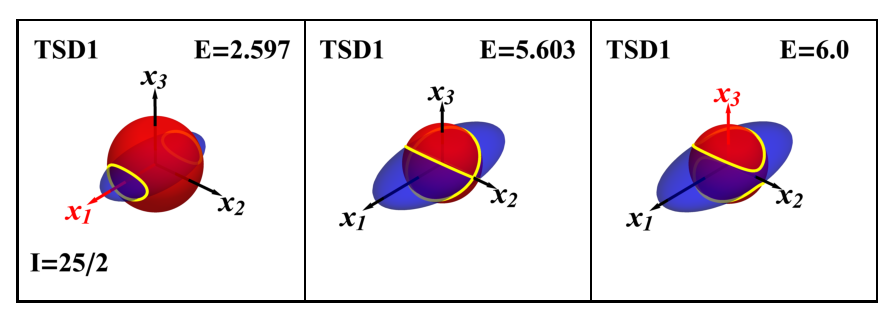
\includegraphics[width=0.9\textwidth]{images/energy_ellipsoids/tsd1_spin1.eps}
    \caption{Image 1}
    \label{fig:image-1}
\end{figure*}

\begin{figure*}
    \centering
    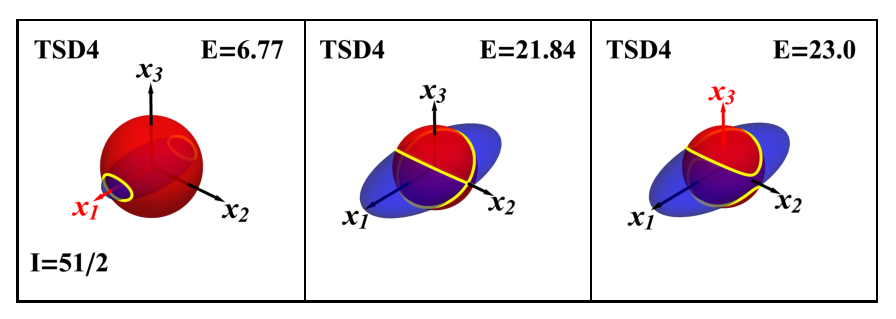
\includegraphics[width=0.9\textwidth]{images/energy_ellipsoids/tsd4_spin2.eps}
    \caption{Image 2}
    \label{fig:image-2}
\end{figure*}

\subsection{Subsection 1}

\lipsum[1-2]

\begin{figure*}
    \centering
    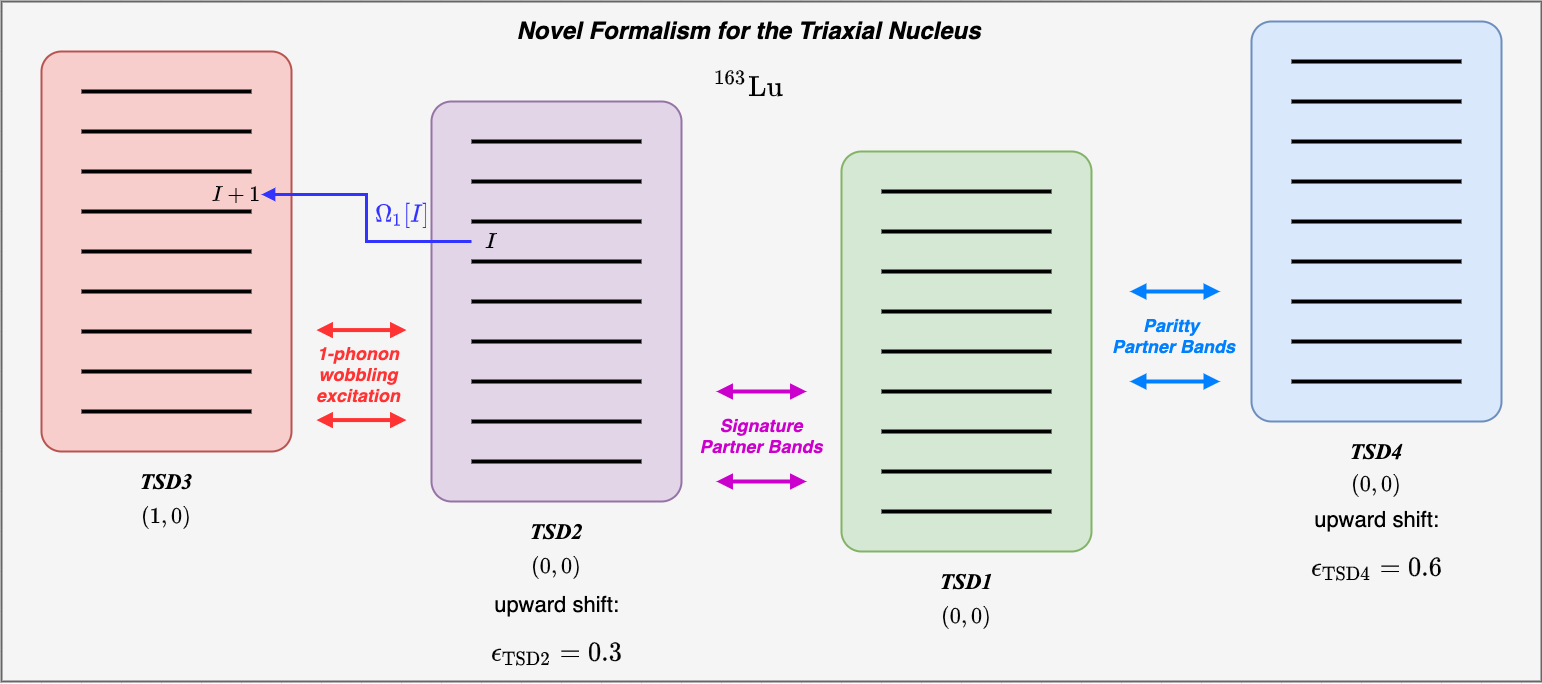
\includegraphics[width=0.9\textwidth]{images/diagrams/double_shift_fit_workflow.png}
    \caption{The workflow involved in the current model.}
    \label{fig:parity-workflow}
\end{figure*}

\lipsum[1-3]

\subsection{Subsection 2}

\lipsum[1-3]

\bibliography{biblio}% Produces the bibliography via BibTeX.

\end{document}